\documentclass{beamer}
\usetheme{Madrid}

\usepackage{ctex}
\usepackage{tikz}

\newcommand{\concept}[1]{{\color{blue} #1}}
\def\E{\mathrm{E}}
\def\D{\mathrm{D}}

\newcommand{\Ga}{\alpha}
\newcommand{\Gb}{\beta}
\newcommand{\Gg}{\gamma}     \newcommand{\GG}{\Gamma}
\newcommand{\Gd}{\delta}     \newcommand{\GD}{\Delta}
\newcommand{\Ge}{\epsilon}
\newcommand{\Gf}{\phi}       \newcommand{\GF}{\Phi}
\newcommand{\Gh}{\theta}
\newcommand{\Gi}{\iota}
\newcommand{\Gk}{\kappa}
\newcommand{\Gl}{\lambda}    \newcommand{\GL}{\Lambda}
\newcommand{\Go}{\omega}     \newcommand{\GO}{\Omega}
\newcommand{\Gs}{\sigma}
\newcommand{\Gt}{\tau}
\newcommand{\Gz}{\zeta}

\title{EM 算法}
\author{祝润天}
\institute{复旦大学计算机科学技术学院}
\date{2024 年 12 月 6 日}

\begin{document}

\begin{frame}
    
    \maketitle

\end{frame}

\begin{frame}
    \frametitle{投硬币实验}

    \begin{columns}
        \begin{column}{0.5\textwidth}
            \centering
            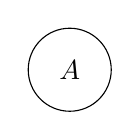
\begin{tikzpicture}
                \draw (0, 0) circle (1.5em) node {$A$};
            \end{tikzpicture}
            \\投出正面:$\Gh_A$
        \end{column}
        \begin{column}{0.5\textwidth}
            \centering
            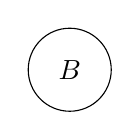
\begin{tikzpicture}
                \draw (0, 0) circle (1.5em) node {$B$};
            \end{tikzpicture}
            \\投出正面:$\Gh_B$
        \end{column}
    \end{columns}
    
    \pause

    \bigskip

    每轮投掷 $10$ 次,结果如下:

    \begin{table}
        \begin{tabular}{c|c|c|c|c|c}
            使用的硬币 & $B$ & $A$ & $A$ & $B$ & $A$ \\\hline
            投掷结果 & $5$ 正 $5$ 反 & $9$ 正 $1$ 反 & $8$ 正 $2$ 反 & $4$ 正 $6$ 反 & $7$ 正 $3$ 反
        \end{tabular}
    \end{table}

    \bigskip

    如何估计 $\Gh_A$ 和 $\Gh_B$?

\end{frame}

\begin{frame}
    \frametitle{投硬币实验}

    \begin{table}
        \begin{tabular}{c|c|c|c|c|c}
            使用的硬币 & $B$ & $A$ & $A$ & $B$ & $A$ \\\hline
            投掷结果 & $5$ 正 $5$ 反 & $9$ 正 $1$ 反 & $8$ 正 $2$ 反 & $4$ 正 $6$ 反 & $7$ 正 $3$ 反
        \end{tabular}
    \end{table}

    \bigskip

    分别用硬币为 $A$ 和 $B$ 的样本求 $\Gh_A$ 和 $\Gh_B$ 的最大似然估计。以 $A$ 为例,设 $X$ 为一次实验中出现正面的个数:

    \begin{itemize}
        \item $X \sim B(10, \Gh_1)$
        \item $X_1 = 9, X_2 = 8, X_3 = 7$
        \item 极大似然估计为 $\hat{\Gh_A} = \frac{\overline{X}}{10} = 0.8$
    \end{itemize}

\end{frame}

\begin{frame}
    \frametitle{投硬币实验}

    如果不知道每次使用的硬币怎么办?(但已知每次等概率从 $A$ 或 $B$ 中选取一枚硬币)

    \begin{table}
        \begin{tabular}{c|c|c|c|c|c}
            使用的硬币 & ? & ? & ? & ? & ? \\\hline
            投掷结果 & $5$ 正 $5$ 反 & $9$ 正 $1$ 反 & $8$ 正 $2$ 反 & $4$ 正 $6$ 反 & $7$ 正 $3$ 反
        \end{tabular}
    \end{table}

    \begin{itemize}
        \item 将使用的硬币也作为未知参数估计
        \begin{itemize}
            \item 难以求得解析解
        \end{itemize}
        \item 用迭代算法估计
    \end{itemize}

\end{frame}

\begin{frame}
    \frametitle{EM 算法}

    \begin{table}
        \begin{tabular}{c|c|c|c|c|c}
            使用的硬币 & $z_1$ & $z_2$ & $z_3$ & $z_4$ & $z_5$ \\\hline
            投掷结果 & $5$ 正 $5$ 反 & $9$ 正 $1$ 反 & $8$ 正 $2$ 反 & $4$ 正 $6$ 反 & $7$ 正 $3$ 反
        \end{tabular}
    \end{table}

    \begin{itemize}
        \item 随机初始化 $\Gh_A$ 和 $\Gh_B$
        \item 例:$\Gh_A = 0.5$, $\Gh_B = 0.6$
        \item 计算 $z_1$ 和 $z_2$ 的最大似然估计
    \end{itemize}

\end{frame}

\begin{frame}
    \frametitle{EM 算法}

    $\Gh_A = 0.5, \Gh_B = 0.6$

    \begin{itemize}
        \item 若第一轮使用硬币 $A$:$P(5 \text{正} 5 \text{反}) = {10 \choose 5}\Gh_A^{5}(1 - \Gh_A)^{5} \approx 0.246$
        \item 若第一轮使用硬币 $B$:$P(5 \text{正} 5 \text{反}) = {10 \choose 5}\Gh_B^{5}(1 - \Gh_B)^{5} \approx 0.201$
    \end{itemize}

    根据最大似然原理,$\hat{z_1} = A$

    \begin{table}
        \begin{tabular}{c|c|c|c|c|c}
            使用的硬币 & $z_1 = A$ & $z_2 = B$ & $z_3 = B$ & $z_4 = A$ & $z_5 = B$ \\\hline
            投掷结果 & $5$ 正 $5$ 反 & $9$ 正 $1$ 反 & $8$ 正 $2$ 反 & $4$ 正 $6$ 反 & $7$ 正 $3$ 反
        \end{tabular}
    \end{table}

\end{frame}

\begin{frame}
    \frametitle{EM 算法}

    \begin{table}
        \begin{tabular}{c|c|c|c|c|c}
            使用的硬币 & $z_1 = A$ & $z_2 = B$ & $z_3 = B$ & $z_4 = A$ & $z_5 = B$ \\\hline
            投掷结果 & $5$ 正 $5$ 反 & $9$ 正 $1$ 反 & $8$ 正 $2$ 反 & $4$ 正 $6$ 反 & $7$ 正 $3$ 反
        \end{tabular}
    \end{table}

    使用预测的结果重新用最大似然方法估计 $\Gh_A$ 和 $\Gh_B$ 的值

    \[\Gh_A = 0.5, \Gh_B = 0.8\]

\end{frame}

\begin{frame}
    \frametitle{EM 算法}

    用新的 $\Gh_A$ 和 $\Gh_B$ 再次估计每一轮使用的硬币

    \begin{table}
        \begin{tabular}{c|c|c|c|c|c}
            使用的硬币 & $z_1 = A$ & $z_2 = B$ & $z_3 = B$ & $z_4 = A$ & $z_5 = B$ \\\hline
            投掷结果 & $5$ 正 $5$ 反 & $9$ 正 $1$ 反 & $8$ 正 $2$ 反 & $4$ 正 $6$ 反 & $7$ 正 $3$ 反
        \end{tabular}
\end{table}

    结果不变,则算法结束

\end{frame}

\begin{frame}
    \frametitle{EM 算法的改进}

    估计 $z_i$ 的值 $\rightarrow$ 估计 $z_i$ 的概率分布

    \pause

    \[\begin{split}
        & P(z_1 = A \vert X_1 = 5) \\
        = & \frac{P(z_1 = A)P(X_1 = 5 \vert z_1 = A)}{P(z_1 = A)P(X_1 = 5 \vert z_1 = A) + P(z_1 = B)P(X_1 = 5 \vert z_1 = B)} \\
        \approx & \frac{0.5\times 0.246}{0.5\times 0.246 + 0.201} \\
        \approx & 0.55
    \end{split}\]

    \[\begin{array}{c|c|c}
        z & A & B \\\hline
        P(z_1 = z) & 0.55 & 0.45
    \end{array}\]

\end{frame}

\begin{frame}
    \frametitle{EM 算法的改进}

    用 $z_i$ 的概率分布估计 $\Gh_A$ 和 $\Gh_B$
    
    \begin{figure}
        \centering
        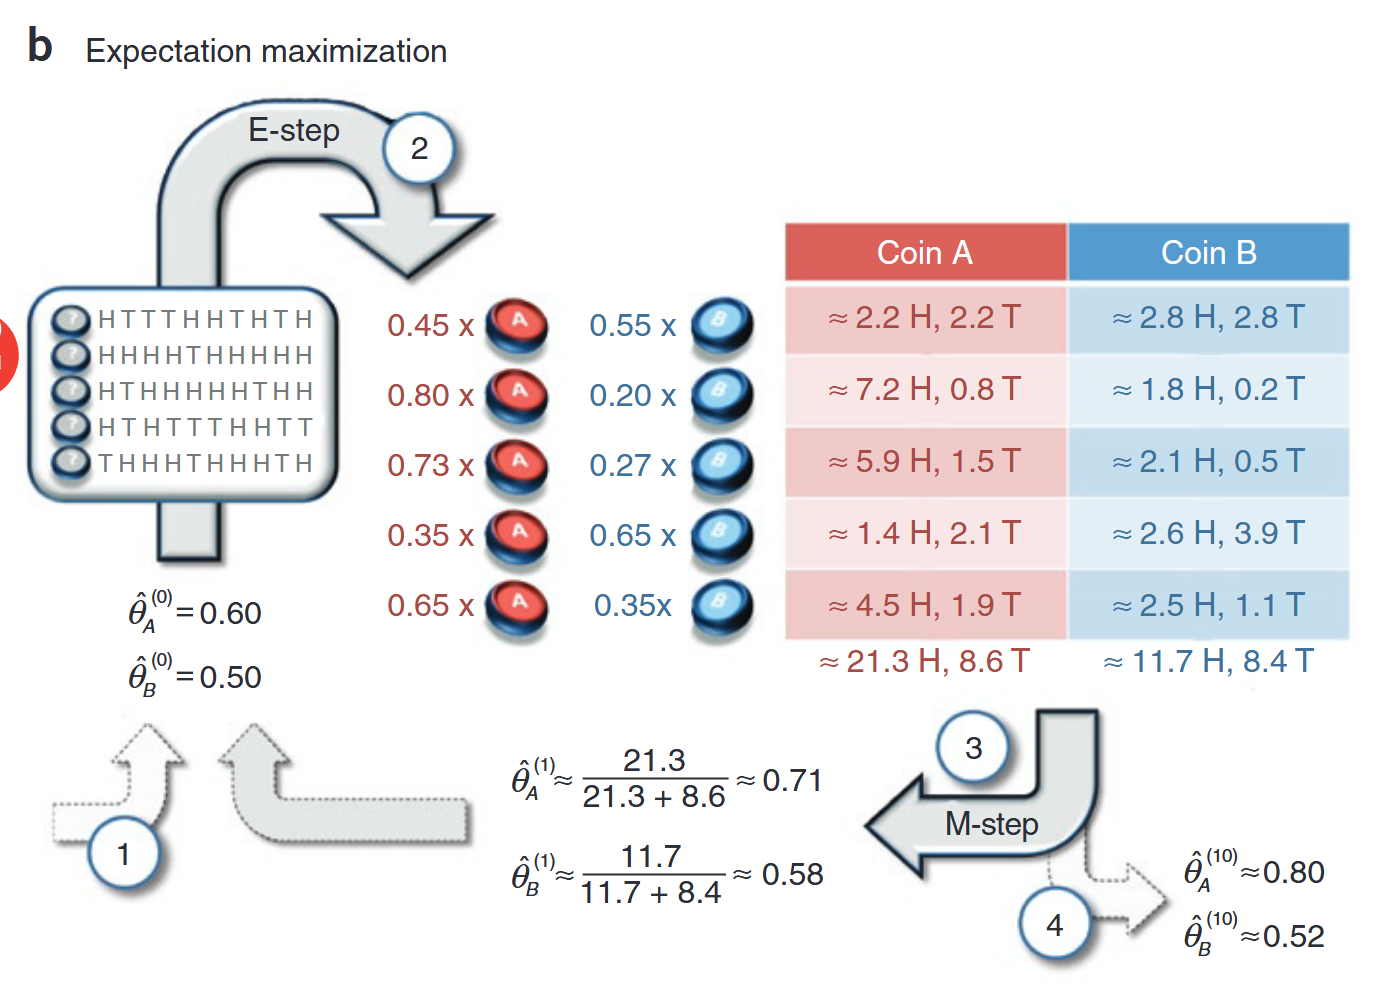
\includegraphics[width=.8\textwidth]{res/em.png}
    \end{figure}

\end{frame}

\begin{frame}
    \frametitle{数学推导}

    假设样本集为 $x_1, \dots, x_n$,每个样本 $x_i$ 都有一个未知的隐变量 $z_i$。希望用极大似然估计求解参数 $\Gh$。则似然函数为

    \[L(x, z, \Gh) = \prod_{i = 1}^{n} p(x_i, \Gh) =  \prod_{i = 1}^{n} \sum_{z_i}p(x_i, z_i, \Gh)\]

    则

    \[\ln L(x, z, \Gh) = \sum_{i = 1}^{n}\ln \sum_{z_i} p(x_i, z_i, \Gh)\]

    设 $z_i$ 的概率分布为 $Q_i(z_i)$,则

    \[\ln L(x, z, \Gh) = \sum_{i = 1}^{n}\ln \sum_{z_i} Q_i(z_i) \frac{p(x_i, z_i, \Gh)}{Q_i(z_i)} = \sum_{i = 1}^{n}\ln \E(\frac{p(x_i, z_i, \Gh)}{Q_i(z_i)})\]

\end{frame}

\begin{frame}
    \frametitle{詹森不等式}

    如果 $f$ 是凸函数,$X$ 是随机变量,则 $\E[f(X)]>=f(\E[X])$。

    如果 $f$ 是严格凸函数,当且仅当 $P(X = \E[X]) = 1$ 时上式取等。
    
    \begin{figure}
        \centering
        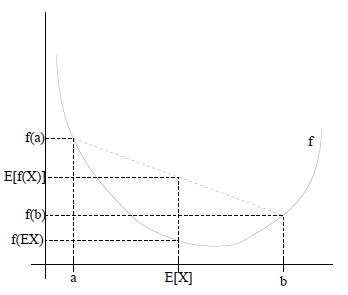
\includegraphics[width=.5\textwidth]{res/jensen.png}
    \end{figure}

\end{frame}

\begin{frame}
    \frametitle{数学推导}

    \[\begin{split}
        \ln L(x, z, \Gh) = & \sum_{i = 1}^{n}\ln \E(\frac{p(x_i, z_i, \Gh)}{Q_i(z_i)}) \\
        \geq & \sum_{i = 1}^{n} \E(\ln \frac{p(x_i, z_i, \Gh)}{Q_i(z_i)}) \\
        = & \sum_{i = 1}^{n}\sum_{z_i} Q_i(z_i) \ln \frac{p(x_i, z_i, \Gh)}{Q_i(z_i)}
    \end{split}\]

\end{frame}

\begin{frame}
    \frametitle{数学推导}
    
    何时取等? $P(X = \E[X]) = 1$(粗略地讲,$X$ 为常数)。此时,

    \[\frac{p(x_i, z_i, \Gh)}{Q_i(z_i)} = c\]
    \[\sum_{z_i} p(x_i, z_i, \Gh) = c \sum_{z_i} Q_i(z_i) = c\]

    \[\begin{split}
        Q_i(z_i) = & \frac{p(x_i, z_i, \Gh)}{c} \\
        = & \frac{p(x_i, z_i, \Gh)}{\sum_{z_i} p(x_i, z_i, \Gh)} \\
        = & \frac{p(x_i, z_i, \Gh)}{p(x_i, \Gh)} \\
        = & P(z_i \vert x_i, \Gh)
    \end{split}\]

\end{frame}

\begin{frame}
    \frametitle{EM 算法图示}

    \[\begin{split}
        L(\Gh) = & \sum_{i = 1}^{n}\ln \E(\frac{p(x_i, z_i, \Gh)}{Q_i(z_i)}) \geq \sum_{i = 1}^{n} \E(\ln \frac{p(x_i, z_i, \Gh)}{Q_i(z_i)}) = J(Q)
    \end{split}\]
    
    \begin{figure}
        \centering
        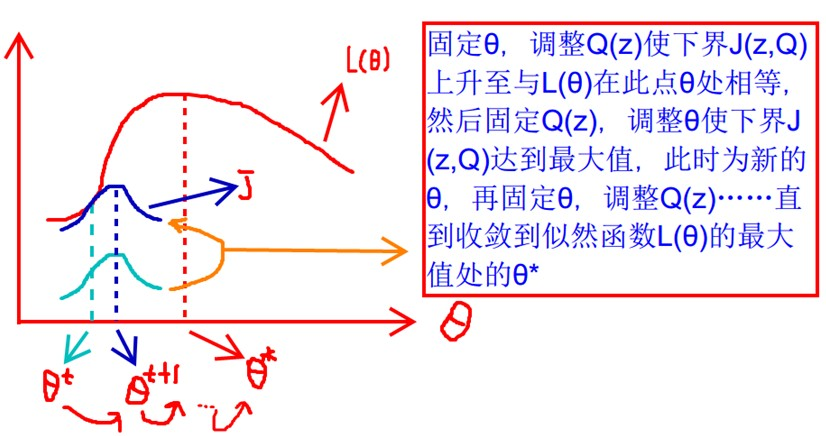
\includegraphics[width=.8\textwidth]{res/em_function.png}
    \end{figure}

\end{frame}

\begin{frame}
    \frametitle{另一视角:坐标上升法}

    \[J(Q, \Gh) = \sum_{i = 1}^{n}\sum_{z_i}Q_i(z_i)\ln \frac{p(x_i, z_i, \Gh)}{Q_i(z_i)}\]

    \begin{figure}
        \centering
        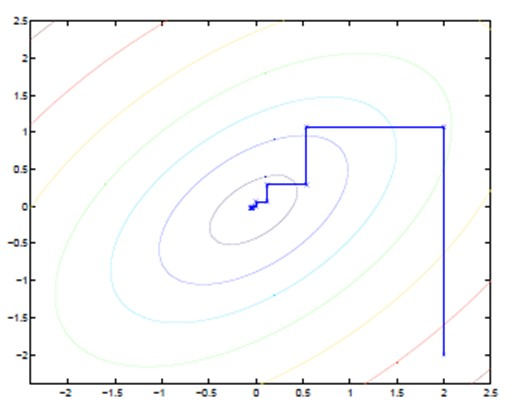
\includegraphics[width=.6\textwidth]{res/coordinate_ascent.png}
    \end{figure}

\end{frame}

\end{document}